\documentclass[11pt,a4paper]{article}

% ── Compilar con: tectonic x5_documento.tex  (motor XeTeX, UTF-8 nativo) ──
\usepackage{fontspec}
\usepackage{amsmath,amssymb}
\usepackage[margin=2.2cm]{geometry}
\usepackage{xcolor}
\usepackage{tikz}
\usetikzlibrary{positioning,arrows.meta,shapes.geometric,fit,backgrounds,calc}
\usepackage{booktabs}
\usepackage{listings}
\usepackage{enumitem}
\usepackage[hidelinks]{hyperref}

% ── Colores ──
\definecolor{cazul}{HTML}{2C5F8A}
\definecolor{cverde}{HTML}{2E8B57}
\definecolor{cnaranja}{HTML}{C1660A}
\definecolor{cgris}{HTML}{5B6770}
\definecolor{cfondo}{HTML}{F2F5F8}
\definecolor{ccodefondo}{HTML}{F6F8FA}

% ── Estilo de código ──
\lstset{
  basicstyle=\ttfamily\small,
  backgroundcolor=\color{ccodefondo},
  frame=single,
  rulecolor=\color{cgris!40},
  breaklines=true,
  columns=fullflexible,
  keepspaces=true,
  showstringspaces=false,
  xleftmargin=6pt,
  framexleftmargin=4pt,
}
\newcommand{\code}[1]{\texttt{#1}}

% ── Estilos TikZ ──
\tikzset{
  caja/.style={rectangle, rounded corners=3pt, draw=cazul, fill=cazul!8,
    text width=3.1cm, align=center, minimum height=1cm, font=\small},
  cajav/.style={rectangle, rounded corners=3pt, draw=cverde, fill=cverde!8,
    text width=3.1cm, align=center, minimum height=1cm, font=\small},
  cajan/.style={rectangle, rounded corners=3pt, draw=cnaranja, fill=cnaranja!8,
    text width=3.1cm, align=center, minimum height=1cm, font=\small},
  cajag/.style={rectangle, rounded corners=3pt, draw=cgris, fill=cgris!8,
    text width=2.6cm, align=center, minimum height=0.9cm, font=\small},
  flecha/.style={-{Stealth[length=3mm]}, thick, draw=cgris},
  etq/.style={font=\footnotesize\itshape, text=cgris},
}

\title{\vspace{-1cm}\textbf{X5 — El cerebro de Alginvesting}\\[4pt]
  \large Surrogate model para ajuste dinámico de parámetros\\[2pt]
  \normalsize\color{cgris} Guía técnica y conceptual (con peras y manzanas)}
\author{Proyecto Alginvesting}
\date{\today}

\begin{document}
\maketitle
\thispagestyle{empty}

\begin{center}
\begin{minipage}{0.85\textwidth}
\color{cgris}\small
Este documento fusiona \code{x5\_plan.md} y \code{x5\_plan\_redes\_neuronales.md}.
Explica \emph{qué} hace X5, \emph{cómo} está construido (LightGBM y FT-Transformer),
\emph{cómo} se entrena desde cero con backtesting paralelo y \emph{cómo} recomienda los
parámetros de trading. Pensado para leerse impreso.
\end{minipage}
\end{center}

\tableofcontents
\newpage

% ═══════════════════════════════════════════════════════════════════
\section{Qué es X5 y por qué es el cerebro}

Alginvesting coloca órdenes de compra en soportes calculados por X0 y las gestiona con X1.
Esos módulos dependen de \textbf{parámetros de configuración} (\code{K}, \code{N\_EXP},
\code{LAMBDA}, \code{n\_sizes\_ejecucion}, \code{LOTAJES\_M}, \code{A}, \code{B},
\code{PERDIDA\_MAX}). Hoy son fijos. El problema: los parámetros óptimos \textbf{cambian con
el régimen de mercado} (una caída fuerte de BTC pide menos exposición que un mercado lateral).

\textbf{X5 es un \emph{surrogate model}}: un modelo que predice el \textbf{retorno esperado} de
una operación dado (1) el contexto de mercado y (2) los parámetros usados. Con esa predicción,
en inferencia \textbf{invierte la pregunta}: ``con el mercado de hoy fijo, ¿qué parámetros
maximizan el retorno predicho?''. Ese set se escribe en
\code{config/active\_parameters.json}, que X1 puede leer.

\begin{center}
\resizebox{\textwidth}{!}{%
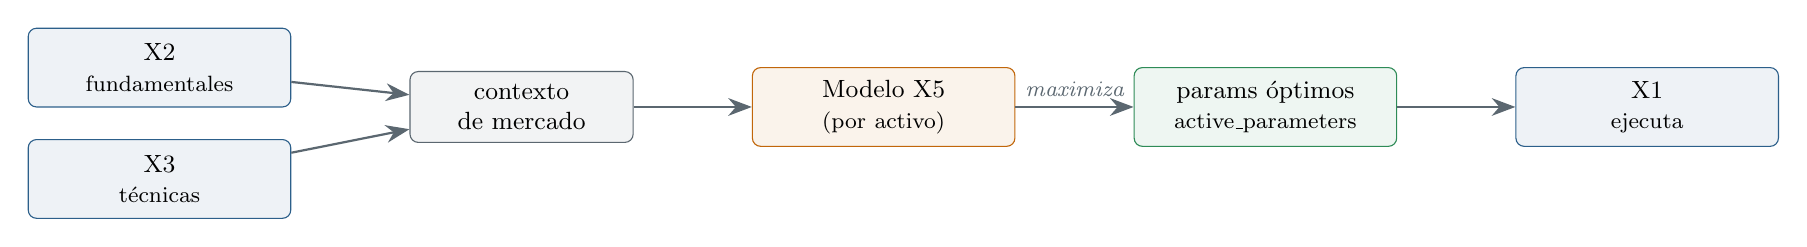
\begin{tikzpicture}[node distance=1.0cm and 1.5cm]
  \node[caja] (x2) {X2\\\footnotesize fundamentales};
  \node[caja, below=0.4cm of x2] (x3) {X3\\\footnotesize técnicas};
  \node[cajag, right=of x2, yshift=-0.5cm] (ctx) {contexto\\de mercado};
  \node[cajan, right=of ctx] (modelo) {Modelo X5\\\footnotesize (por activo)};
  \node[cajav, right=of modelo] (params) {params óptimos\\\footnotesize active\_parameters};
  \node[caja, right=of params] (x1) {X1\\\footnotesize ejecuta};

  \draw[flecha] (x2) -- (ctx);
  \draw[flecha] (x3) -- (ctx);
  \draw[flecha] (ctx) -- (modelo);
  \draw[flecha] (modelo) -- (params) node[midway, above, etq] {maximiza};
  \draw[flecha] (params) -- (x1);
\end{tikzpicture}%
}
\end{center}

\textbf{Todo es por activo.} X5 entrena un modelo independiente para BTCUSD, ETHUSD, TSLA,
GOOGL, NVDA y AMZN. Cada uno tiene sus propios datos, su propio modelo y su propia ``fase''.

% ═══════════════════════════════════════════════════════════════════
\section{La analogía del chef}

Imagina un chef que cocinó miles de platos (operaciones) en cocinas de distintas condiciones
(mercados). Lleva un cuaderno: qué ingredientes usó (parámetros), cómo estaba la cocina
(contexto), y cómo quedó el plato (retorno). Con suficiente experiencia, puede predecir:
``con esta receta en una cocina así, el plato sale 8/10''.

\begin{itemize}[leftmargin=1.4em]
  \item \textbf{El chef} = el modelo de X5.
  \item \textbf{El cuaderno de recetas} = el \emph{store} de trades (\code{resources/x5/\{ACTIVO\}\_store.csv}).
  \item \textbf{Una receta} = un set de parámetros.
  \item \textbf{Preguntar la mejor receta para hoy} = inferencia (\code{--infer}).
\end{itemize}

Al principio el chef \textbf{no sabe nada}: hay que hacerlo cocinar mucho (backtesting) para
llenar el cuaderno, y recién entonces puede estudiar y recomendar.

% ═══════════════════════════════════════════════════════════════════
\section{Qué entra y qué sale del modelo}

\subsection{Inputs (\textasciitilde240 features, vector de tamaño fijo)}

Cada fila del cuaderno es una operación. Sus columnas:
\begin{itemize}[leftmargin=1.4em,itemsep=1pt]
  \item \textbf{Contexto X2+X3 en dos momentos}: al colocar el buy limit (\textbf{OE}) y al
  ejecutarse la orden (\textbf{OA}). Entre ambos pueden pasar días, y el mercado cambia.
  \item \textbf{Parámetros de config} activos en esa operación (los ``ingredientes'').
  \item \textbf{Features temporales}: hora, día de semana, mes, proximidad a festivos US.
  \item \textbf{Estado del portfolio}: cuántas posiciones abiertas, exposición, retorno flotante.
\end{itemize}
El contexto de \textbf{cierre (OC) NO entra} al modelo: es información del futuro, no disponible
en inferencia.

\subsection{Outputs (3 objetivos que el modelo predice)}

\begin{center}
\begin{tabular}{@{}lll@{}}
\toprule
\textbf{Nombre en el código} & \textbf{Qué mide} & \textbf{En qué filas} \\
\midrule
\code{retorno\_pct} & retorno \% de la operación cerrada & \code{oc} \\
\code{pnl\_flotante\_activo} & P\&L flotante de posiciones abiertas & \code{oc} + \code{periodico} \\
\code{pnl\_cerrado\_activo} & P\&L cerrado acumulado del activo & \code{oc} \\
\bottomrule
\end{tabular}
\end{center}

El objetivo que se maximiza en inferencia es configurable; por defecto \code{retorno\_pct}
(la señal más limpia).

% ═══════════════════════════════════════════════════════════════════
\section{Arquitectura que escala con los datos}

X5 no arranca con una arquitectura fija: \textbf{sube de nivel según cuántos datos tenga cada
activo}. La transición es automática y por activo (umbrales en \code{config.py}).

\begin{center}
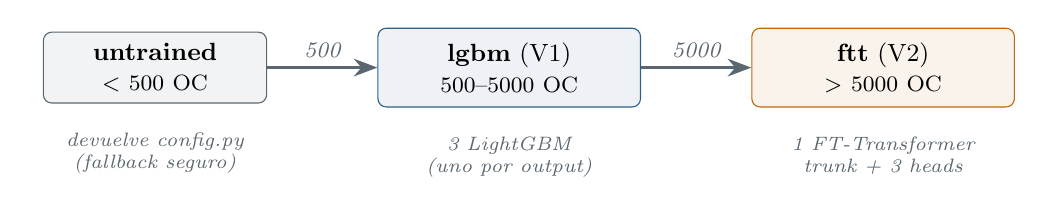
\begin{tikzpicture}[node distance=1.4cm]
  \node[cajag] (u) {\textbf{untrained}\\\footnotesize $<$ 500 OC};
  \node[caja, right=of u] (l) {\textbf{lgbm} (V1)\\\footnotesize 500--5000 OC};
  \node[cajan, right=of l] (f) {\textbf{ftt} (V2)\\\footnotesize $>$ 5000 OC};
  \draw[flecha] (u) -- (l) node[midway,above,etq]{500};
  \draw[flecha] (l) -- (f) node[midway,above,etq]{5000};
  \node[below=0.25cm of u, text width=3cm, align=center, font=\scriptsize\itshape, text=cgris]
    {devuelve config.py\\(fallback seguro)};
  \node[below=0.25cm of l, text width=3cm, align=center, font=\scriptsize\itshape, text=cgris]
    {3 LightGBM\\(uno por output)};
  \node[below=0.25cm of f, text width=3cm, align=center, font=\scriptsize\itshape, text=cgris]
    {1 FT-Transformer\\trunk + 3 heads};
\end{tikzpicture}
\end{center}

\noindent Estado actual: el store está vacío, así que los 6 activos están en \textbf{untrained}.
El objetivo de la Fase 1 es recolectar datos para pasar a \code{lgbm}.

% ═══════════════════════════════════════════════════════════════════
\section{El store: el cuaderno de recetas}

El store tiene \textbf{dos tipos de fila}, distinguidas por \code{tipo\_registro}:

\begin{center}
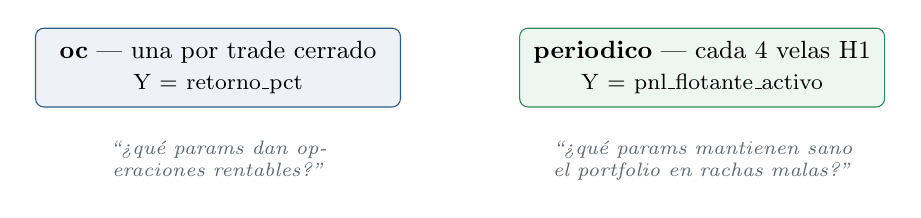
\begin{tikzpicture}[node distance=0.6cm]
  \node[caja, text width=4.4cm] (oc) {\textbf{oc} — una por trade cerrado\\\footnotesize Y = retorno\_pct};
  \node[cajav, text width=4.4cm, right=1.5cm of oc] (per) {\textbf{periodico} — cada 4 velas H1\\\footnotesize Y = pnl\_flotante\_activo};
  \node[below=0.3cm of oc, text width=4.6cm, align=center, font=\scriptsize\itshape, text=cgris]
    {``¿qué params dan operaciones rentables?''};
  \node[below=0.3cm of per, text width=4.6cm, align=center, font=\scriptsize\itshape, text=cgris]
    {``¿qué params mantienen sano el portfolio en rachas malas?''};
\end{tikzpicture}
\end{center}

\textbf{Por qué los dos:} si solo se guardan filas al cerrar órdenes, durante una caída
sostenida (posiciones en rojo, ninguna cierra) el modelo no recibe señal justo cuando más
importa. Los registros periódicos capturan ese deterioro aunque no haya OC.

% ═══════════════════════════════════════════════════════════════════
\section{V1 — LightGBM: el comité de expertos}

\textbf{Gradient Boosting} entrena muchos árboles de decisión en secuencia, donde cada árbol
corrige los errores del anterior.

\begin{center}
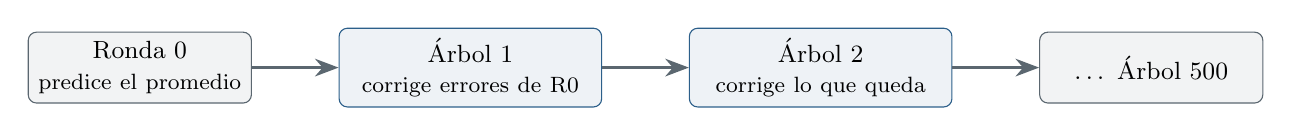
\begin{tikzpicture}[node distance=1.1cm]
  \node[cajag] (r0) {Ronda 0\\\footnotesize predice el promedio};
  \node[caja, right=of r0] (r1) {Árbol 1\\\footnotesize corrige errores de R0};
  \node[caja, right=of r1] (r2) {Árbol 2\\\footnotesize corrige lo que queda};
  \node[cajag, right=of r2] (rn) {\ldots\ Árbol 500};
  \draw[flecha] (r0) -- (r1);
  \draw[flecha] (r1) -- (r2);
  \draw[flecha] (r2) -- (rn);
\end{tikzpicture}
\end{center}

\[
\text{retorno\_predicho} = \text{promedio} + \sum_{i=1}^{500} \text{corrección}_i
\]

Cada árbol es simple (``si RSI $<$ 50 corrige $+1.5\%$''). La potencia viene de acumular
cientos de correcciones pequeñas. Es robusto con pocos datos ($<$50k filas), no requiere
normalización y es interpretable. Su contra: \textbf{no es diferenciable}, así que la
búsqueda de params en inferencia usa Optuna (más lenta que gradient ascent).

% ═══════════════════════════════════════════════════════════════════
\section{V2 — FT-Transformer: atención sobre features}

Cuando el store crece ($>$5000 OC), el salto natural es el \textbf{FT-Transformer}
(Feature Tokenizer + Transformer).

\subsection{Paso 1 — Feature Tokenizer: cada número se vuelve un vector}

En una red común, cada feature entra como un número. El tokenizer la convierte en un
\textbf{vector} (embedding) propio y aprendido:
\[
\text{embedding}_i = \text{valor}_i \times W_i + b_i
\]

\begin{center}
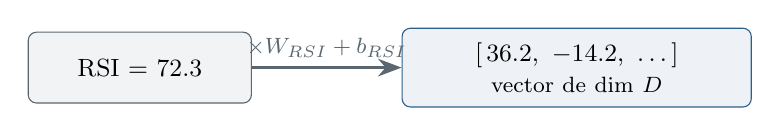
\begin{tikzpicture}[node distance=0.9cm]
  \node[cajag] (rsi) {RSI = 72.3};
  \node[caja, right=1.9cm of rsi, text width=4.2cm] (emb) {$[\,36.2,\ -14.2,\ \ldots\,]$\\\footnotesize vector de dim $D$};
  \draw[flecha] (rsi) -- (emb) node[midway,above,etq]{$\times W_{RSI}+b_{RSI}$};
\end{tikzpicture}
\end{center}

Así ``RSI = 72'' \emph{significa} algo distinto que ``RSI = 30'', y esa diferencia queda
codificada en el vector. Cada feature tiene sus propios $W_i, b_i$ aprendidos.

\subsection{Paso 2 — Atención: las features ``se hablan entre sí''}

\textbf{La reunión de equipo.} Cada feature es una persona. En una red normal, cada una escribe
su conclusión y la manda a la salida sin escuchar a las demás. En un Transformer, \textbf{antes
de concluir, cada persona escucha a las otras y ajusta lo que dirá}. RSI puede pensar: ``soy
alto, normalmente mala señal — pero oí que la volatilidad también es alta y el fundamental es
sano; quizás no sea tan malo''.

El mecanismo usa tres vectores por feature: \textbf{Q} (qué busco), \textbf{K} (qué ofrezco),
\textbf{V} (lo que comparto). RSI mide su afinidad con cada compañera con el producto
$Q_{RSI}\cdot K_j$, normaliza con \emph{softmax}, y arma su nuevo embedding como suma
ponderada de los $V_j$:

\begin{center}
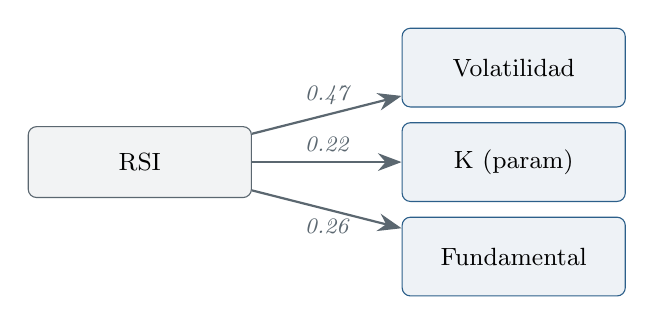
\begin{tikzpicture}[node distance=0.7cm and 1.9cm]
  \node[cajag] (rsi) {RSI};
  \node[caja, right=of rsi, yshift=1.2cm, text width=2.6cm] (vol) {Volatilidad};
  \node[caja, right=of rsi, text width=2.6cm] (k) {K (param)};
  \node[caja, right=of rsi, yshift=-1.2cm, text width=2.6cm] (fund) {Fundamental};
  \draw[flecha] (rsi) -- (vol) node[midway,above,etq]{0.47};
  \draw[flecha] (rsi) -- (k)   node[midway,above,etq]{0.22};
  \draw[flecha] (rsi) -- (fund) node[midway,below,etq]{0.26};
\end{tikzpicture}
\end{center}

\textbf{Multi-head}: el mecanismo corre varias veces en paralelo (cabezas), cada una captura un
tipo de relación (técnicas entre sí, params$\times$contexto, riesgo). Se apilan varias capas:
la capa 1 ve relaciones directas, la 2 relaciones entre representaciones ya contextualizadas,
etc. Para datos tabulares, 2--4 capas bastan.

\subsection{Multi-head de salida: predecir 3 cosas a la vez}

\begin{center}
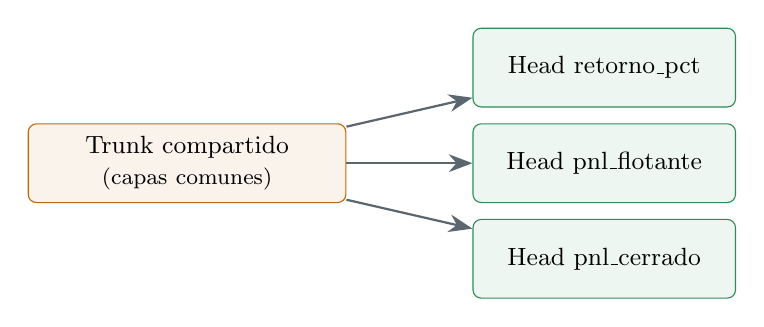
\begin{tikzpicture}[node distance=1.0cm]
  \node[cajan, text width=3.8cm] (trunk) {Trunk compartido\\\footnotesize (capas comunes)};
  \node[cajav, above right=0.2cm and 1.6cm of trunk] (h1) {Head retorno\_pct};
  \node[cajav, right=1.6cm of trunk] (h2) {Head pnl\_flotante};
  \node[cajav, below right=0.2cm and 1.6cm of trunk] (h3) {Head pnl\_cerrado};
  \draw[flecha] (trunk) -- (h1);
  \draw[flecha] (trunk) -- (h2);
  \draw[flecha] (trunk) -- (h3);
\end{tikzpicture}
\end{center}

Como un médico que hace una revisión (el trunk) y da tres diagnósticos (los heads). Compartir
el trunk actúa como regularización: el modelo no puede sobreajustarse a una sola señal ruidosa
si debe explicar tres a la vez.

% ═══════════════════════════════════════════════════════════════════
\section{Inferencia: encontrar los parámetros óptimos}

Con el contexto de hoy \textbf{fijo}, se buscan los params que maximizan el retorno predicho.

\begin{itemize}[leftmargin=1.4em]
  \item \textbf{LightGBM (no diferenciable)} $\to$ \textbf{Optuna}: un optimizador bayesiano que
  aprende qué zonas del espacio de params son prometedoras y concentra ahí sus intentos
  (\textasciitilde200 trials). Es como pedirle al comité que evalúe 200 recetas y elija la mejor.
  \item \textbf{FT-Transformer (diferenciable)} $\to$ \textbf{gradient ascent}: se calcula
  ``¿en qué dirección mover los params sube el retorno?'' y se avanza en esa dirección, con
  el contexto fijo. Como subir una colina con los ojos vendados tanteando la pendiente. Se
  repite desde varios puntos de inicio para no quedar en un máximo local.
\end{itemize}

\textbf{Airbag}: independiente del modelo, si el precio cayó más de un umbral (8\% crypto,
5\% acciones) en las últimas 4 velas H1, se fuerzan \code{LOTAJES\_M} y \code{n\_sizes} al
mínimo. Es el último recurso; la idea es que el modelo aprenda a ser conservador antes de que
el airbag se dispare.

% ═══════════════════════════════════════════════════════════════════
\section{El sesgo de selección y la exploración}

\textbf{El problema más sutil.} El cuaderno solo contiene operaciones hechas con los params que
el sistema creía ``buenos''. Nunca vemos qué habría pasado con otros. Es como juzgar cuál es el
mejor restaurante yendo siempre al mismo: al final tienes 200 reseñas de uno y cero del resto.

\textbf{Solución — explorar por ciclo entero.} En el backtesting, un $\sim$30\% de los ciclos
usan params \textbf{aleatorios} (EXPLORE) en vez del mejor conocido (EXPLOIT). Los ciclos
EXPLORE rinden peor a propósito: su valor es enseñarle al modelo \emph{qué no funciona} en cada
régimen. Se aleatoriza por \textbf{ciclo completo} (no vela a vela) para que el modelo pueda
atribuir el resultado al contexto sin ruido.

% ═══════════════════════════════════════════════════════════════════
\section{Cómo se ejecuta desde cero (recolección paralela)}

Con el store vacío, el paso principal es \code{--recolectar}: lanza \textbf{un worker por activo
en paralelo}; cada uno corre ciclos de backtesting, y al cruzar 500 OC entrena su propio modelo.

\begin{center}
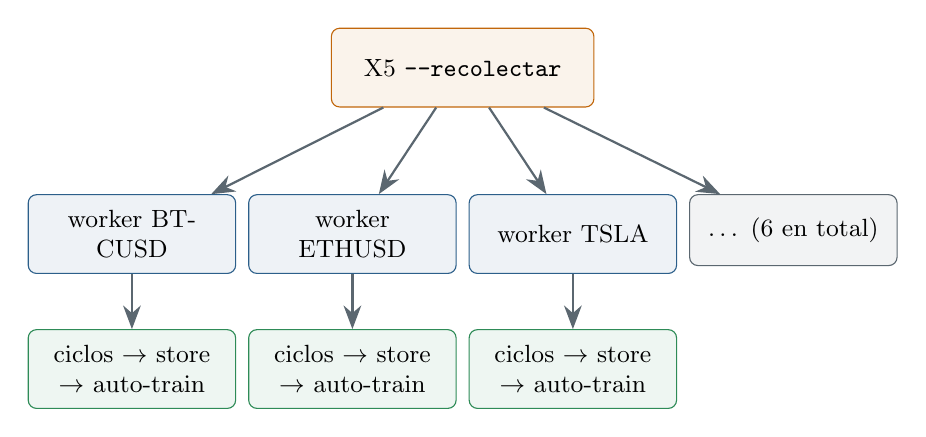
\begin{tikzpicture}[node distance=0.45cm]
  \node[cajan] (x5) {X5 \code{-{}-recolectar}};
  \node[caja, below=1.1cm of x5, xshift=-4.2cm, text width=2.4cm] (w1) {worker BTCUSD};
  \node[caja, below=1.1cm of x5, xshift=-1.4cm, text width=2.4cm] (w2) {worker ETHUSD};
  \node[caja, below=1.1cm of x5, xshift=1.4cm, text width=2.4cm] (w3) {worker TSLA};
  \node[cajag, below=1.1cm of x5, xshift=4.2cm, text width=2.4cm] (wn) {\ldots\ (6 en total)};
  \draw[flecha] (x5) -- (w1);
  \draw[flecha] (x5) -- (w2);
  \draw[flecha] (x5) -- (w3);
  \draw[flecha] (x5) -- (wn);
  \node[cajav, below=0.7cm of w1, text width=2.4cm] (s1) {ciclos $\to$ store $\to$ auto-train};
  \node[cajav, below=0.7cm of w2, text width=2.4cm] (s2) {ciclos $\to$ store $\to$ auto-train};
  \node[cajav, below=0.7cm of w3, text width=2.4cm] (s3) {ciclos $\to$ store $\to$ auto-train};
  \draw[flecha] (w1) -- (s1);
  \draw[flecha] (w2) -- (s2);
  \draw[flecha] (w3) -- (s3);
\end{tikzpicture}
\end{center}

Cada worker usa una carpeta de trabajo aislada (\code{resources\_\{V\}\_\{ACTIVO\}}) para no
chocar con los demás. Cuando termina un ciclo, \textbf{reinicia desde la fecha inicial} con
otros params. Comandos:

\begin{lstlisting}[language=bash]
# 1. estado actual (al inicio: 0 OC, todos untrained)
python scripts/X5_macro_brain.py --status

# 2. generar datos + entrenar (paralelo, 6 activos a la vez)
python scripts/X5_macro_brain.py --recolectar --version V1

# 3. recomendar params -> config/active_parameters.json
python scripts/X5_macro_brain.py --infer
#    (--infer --train  reentrena antes; --infer --activo BTCUSD  solo uno)

# 4. cuando confies en las metricas, activar Fase 2 en config.py:
#    TIPO_EJECUCION = "din"
\end{lstlisting}

\textbf{Fases.} En \textbf{Fase 1} (\code{TIPO\_EJECUCION="est"}) X1 usa \code{config.py} y X5
solo genera datos y recomienda. En \textbf{Fase 2} (\code{"din"}) X1 lee
\code{active\_parameters.json} por activo; los que sigan \code{untrained} caen back a
\code{config.py} automáticamente.

% ═══════════════════════════════════════════════════════════════════
\section{Glosario esencial}

\begin{description}[leftmargin=0pt,itemsep=2pt]
  \item[\textmd{\textbf{Surrogate model}}] Modelo que imita el sistema real para predecir barato el resultado de una operación.
  \item[\textmd{\textbf{Embedding}}] Representar un valor como un vector, para que el modelo lo procese con más riqueza.
  \item[\textmd{\textbf{Atención (Q/K/V)}}] Mecanismo que deja que cada feature ajuste su representación mirando a las demás.
  \item[\textmd{\textbf{Gradient boosting}}] Muchos árboles en secuencia; cada uno corrige el error del anterior. LightGBM lo implementa.
  \item[\textmd{\textbf{Gradient ascent}}] Maximizar una función avanzando en la dirección de su gradiente. Usado en inferencia con FTT.
  \item[\textmd{\textbf{Overfitting}}] El modelo memoriza el pasado en vez de aprender patrones generales.
  \item[\textmd{\textbf{OE / OA / OC}}] Orden en Espera / Orden Abierta / Orden Cerrada.
  \item[\textmd{\textbf{model\_status}}] Estado por activo en el JSON: \code{untrained} / \code{lgbm} / \code{ftt}.
\end{description}

\end{document}
